\documentclass[12pt]{article}
\usepackage{frExamplee}
\usepackage{booktabs}       % professional-quality tables
\usepackage{amsfonts}       % blackboard math symbols
\usepackage{amsmath}
\usepackage{amssymb}
\usepackage{graphicx}
\usepackage{csquotes}
\usepackage{cancel}
\usepackage[backend=biber, style=ieee,]{biblatex}
\usepackage{setspace}
\usepackage[usenames, dvipsnames]{xcolor}
\usepackage{xspace}
\usepackage{caption}
\usepackage{subcaption}
\usepackage{listings}
\usepackage{multirow}
\usepackage{float}
\usepackage{mathrsfs}
\usepackage{wrapfig}
\usepackage{placeins}
\usepackage{algpseudocode}
\usepackage{algorithm}
\usepackage{algorithmicx}
\setstretch{1.4}
\usepackage{hyperref}
\usepackage{calrsfs}
\usepackage{xcolor}
\lstset{
    language=Python,
    basicstyle=\scriptsize\ttfamily,
    keywordstyle=\color{blue},
    commentstyle=\color{green!50!black},
    stringstyle=\color{red},
    showstringspaces=false,
    numbers=left,
    numberstyle=\tiny,
    numbersep=5pt,
    frame=single,
    breaklines=true,
    breakatwhitespace=true,
    tabsize=4,
    captionpos=b
}
\usepackage{setspace}
\usepackage{fancyhdr} 
\fancyhf{}
\cfoot{\thepage}
\pagestyle{fancy}
\renewcommand{\headrulewidth}{0pt}%

\addbibresource{FRtemplates/frExampleRefs.bib}

\title{Practical Applications of the First Law of Thermodynamics}

\author{
Tony Wang\thanks{PRA Section: 3-6, Nov 1st} \\
\texttt{1009027447} \\
\texttt{tonyivt.wang@mail.utoronto.ca} \\
\And
Hyunji Kim \\
\texttt{1008822552} \\
\texttt{hji.kim@mail.utoronto.ca} \\
}
\begin{document}
\maketitle
\begin{abstract}
Originating from the pioneering work of Rudolf Clausius and William Thomson in the mid-19th century, the First Law dictates the fundamental principles that govern energy transformations \autocite{cai2005first}. This lab investigates its applications in an acrylic-tank system involving air flow and heat transfer. Divided into three parts with four trials of distinct temperature and pressure settings, the experiment aims to determine the mass in the tank, quantify heat loss, and calculate the work done by a propeller to discuss its significance \autocite{che}. The calculated values of the mass in the tank are $25.201\pm0.150$, $46.310\pm0.275$, $29.304\pm0.176$, $41.762\pm0.248[g]$ respectively. The calculated values of the specific heat capacity of air are $98.6\pm6.6$, $64.4\pm1.4$, $106\pm7$, $67.2\pm1.4[\frac{kJ}{kgK}]$ respectively. Finally, the calculated values of the work done by a propeller are $81.708\pm0.136$, $136.669\pm0.103$, $81.752\pm0.094$, $137.059\pm0.115[J]$ respectively. These results offer insights into the thermodynamic behavior of the system and their deviation from expected values question the validity of some assumptions.
\end{abstract}
\newpage

\section*{Introduction}
The First Law of Thermodynamics, expressed as 
\begin{equation}
    Q + W = \Delta E
    \label{eq:firstlaw}
\end{equation}
where $Q$ represents heat, $W$ represents work, and $\Delta E$ is the change in internal energy, and serves as the foundation for understanding energy interactions in physical systems. In this experiment, we apply this principle to a system involving air flow and heat transfer\autocite{chandra2016energy}.

\textbf{Part 1} investigates the determination of mass in the left tank using the ideal gas law. By manipulating this law and numerically integrating the mass flow rate curve, the mass of the system can be derived. Experimental procedures involve recording ambient pressure, pressurizing the left tank, and stabilizing pressure and temperature.

\textbf{Part 2} focuses on quantifying heat loss and determining specific heat capacity. Utilizing PID-controlled heaters, the system is maintained at a specified temperature, and the cumulative thermal energy input is calculated. Discussions include calculations of convective heat transfer through cylindrical walls and plates, and the constant volume-specific heat capacity of air at different temperatures.

\textbf{Part 3} examines the work done by a propeller through pump and fan similarity equations, considering changes in internal energy for an adiabatic system. Additionally, fan blade performance equations are employed to analyze the propeller's work. Through achieved values, we quantify the significance of the work contribution by looking at the rate of temperature change as a result of added work.

Each part will be done four times at different temperature and pressure settings for a more thorough investigation. By combining theoretical principles with practical experimentation, this lab aims to provide a comprehensive understanding of thermodynamic concepts and their application in real-world systems. Particular attention will be paid to uncertainties of calculated values, where interpreted uncertainties will be propagated according to standard error propagation techniques \autocite{vern_uncertainties_2000}.

\section*{Method}
\subsection*{Apparatus}
At each workstation, the main setup consisted of two air tanks, sensors, pipes, and valves designed to evaluate the thermodynamic state of the tanks under different conditions. The diagram below depicts the core layout of the workstation, emphasizing the modifiable valves essential for the experiment (Fig. \ref{fig:aparatus}).
\begin{figure}[t!]
\centering
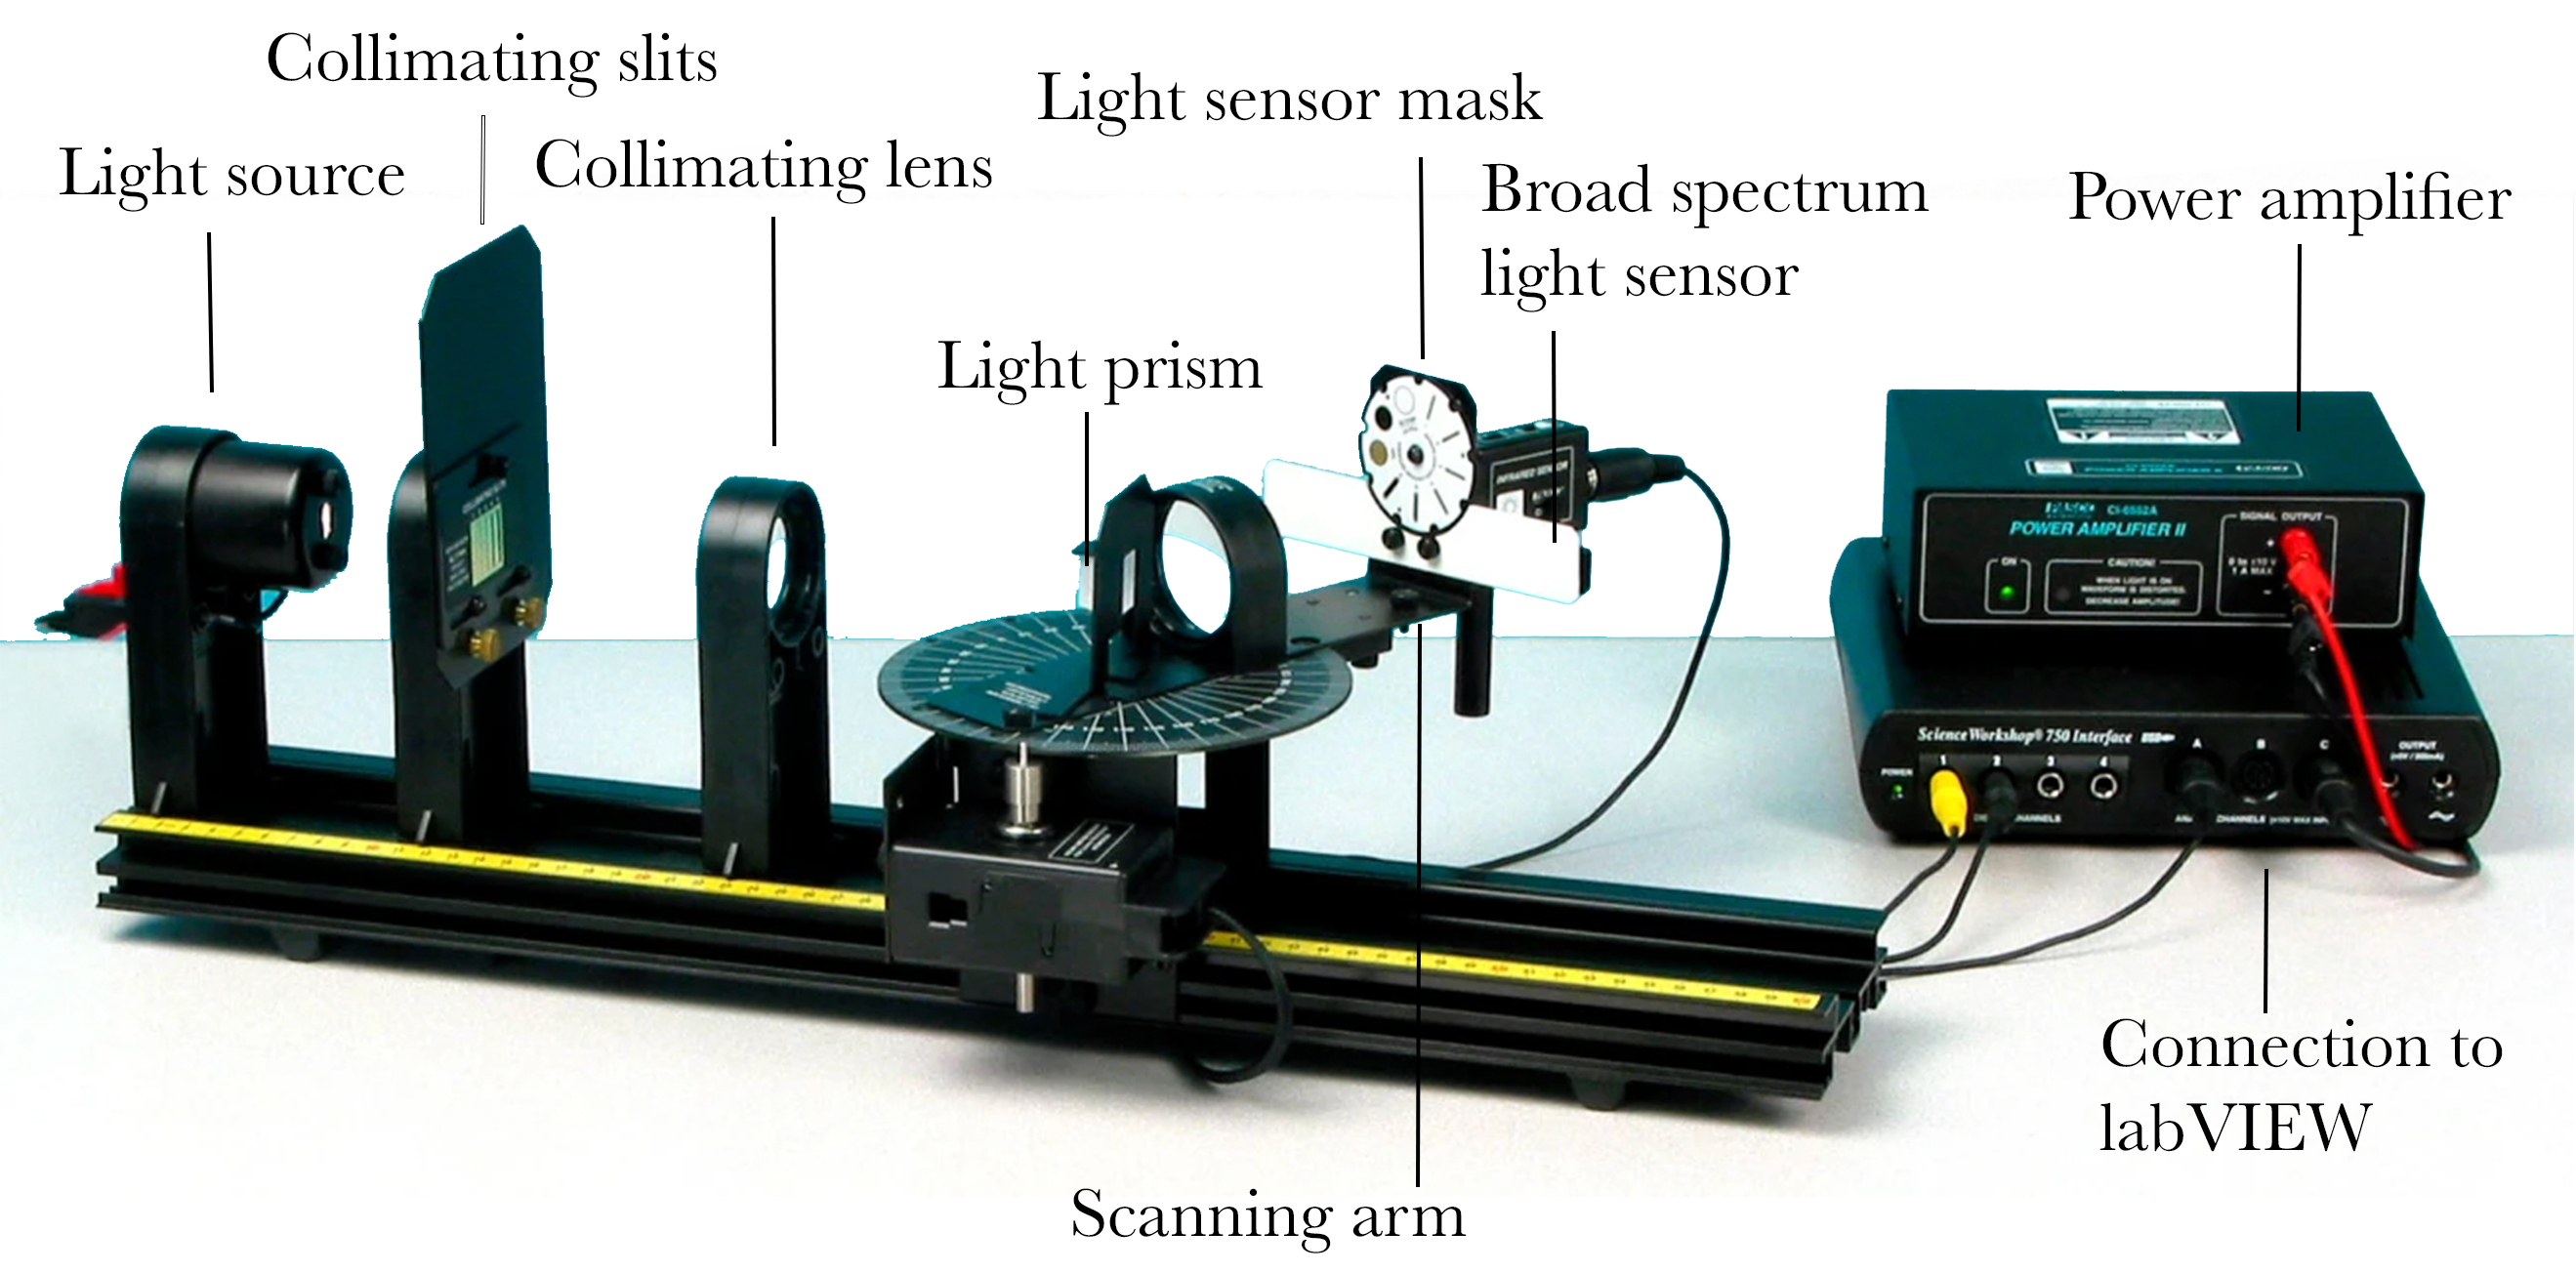
\includegraphics[width=0.7\linewidth]{figure/aparatus.png}
\caption{Drawing of experiment apparatus.}
\label{fig:aparatus}
\end{figure}

\subsection*{Experimental Procedure}
\begin{enumerate}
    \item Mass Determination in the Left Tank \autocite{che}
    \begin{enumerate}
        \item Turn on LabVIEW \autocite{che}, record ambient pressure, and start data collection.
        \item Pressurize the left tank to 40 psi, stabilize, stop recording, and save data.
        \item Reset LabVIEW without emptying the tank.
    \end{enumerate}
    \item Heat Loss and Specific Heat Capacity \autocite{che}
    \begin{enumerate}
        \item Start data collection in LabVIEW, set the temperature to 40°C.
        \item Turn on Heaters, record data after 5 minutes, and save.
        \item Turn off Heaters and cool tanks by running air.
        \item Repeat steps 1-3 for all other trials as in Table \ref{table:procedure}
    \end{enumerate}
    \item Work Done by the Propeller \autocite{che}
    \begin{enumerate}
        \item Start data collection in LabVIEW, set fan conditions using specs.
        \item Record data and save.
        \item Analyze work done by the propeller using equations.
    \end{enumerate}
\end{enumerate}
\begin{table}[h]
  \centering
  \begin{tabular}{|c|c|c|c|}
    \hline
    Trial & Pressure (psig) & Temperature (°C) & Cooling Temperature (°C) \\
    \hline
    1 & 40& 40& 30\\
    2 & 70& 40& 40\\
    3 & 40& 60& 40\\
    4 & 70& 60& 40\\
    \hline
  \end{tabular}
  \caption{Pressure and temperature goals for each trial.}
  \label{table:procedure}
\end{table}

\section*{Results and Discussion}
\subsection*{Part I: Determining mass in the left tank}
The mass of air in the left tank can be determined with:
\begin{equation}
    m_{\rm left}=m_{\rm added}\left[1+\frac{1}{\frac{P_2T_1}{P_1T_2}-1}\right]
    \label{eq:lefttank}
\end{equation}
Numerically integrating the mass flow rate curve (Fig. \ref{fig:mass}) with respect to time, we deduce that we have added $m_{\rm added}=23.6\pm0.5[g]$ by pressurizing the left tank. Given equation (\ref{eq:lefttank}), we arrive at $m_{\rm left}=25.2\pm0.5[g]$ for Trial 1. Similarly, we can do the same for the rest of the trials as shown in Table \ref{table:mass}. Here, all uncertainties are merely determined given the amount of significant figures data from LABVIEW \autocite{che} provides. Error from software and associated hardware are not given and our assumptions may yield incorrect uncertainty values and hence change how we interpret the correctness of calculated values. We also assume that the pressurized air is an ideal gas which is not the case, which will also lead to errors in computed results.
\begin{figure}[t!]
\centering
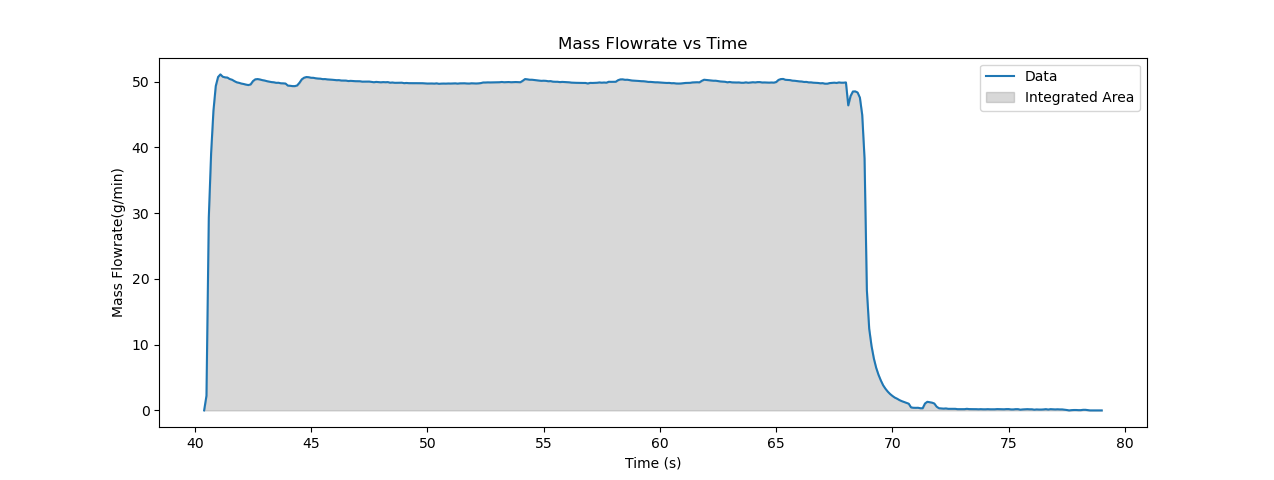
\includegraphics[width=0.9\linewidth]{figure/mass.png}
\caption{Sample mass flowrate curve integrated to find $m_{\rm added}$}
\label{fig:mass}
\end{figure}
\begin{table}[h]
  \centering
  \begin{tabular}{|c|c|c|c|}
    \hline
    Trial & $m_{\rm added}[g]$ & $m_{\rm left}[g]$\\
    \hline
    $1 $& $23.603\pm0.005$ & $25.201\pm0.150$\\
    $2 $& $45.809\pm0.005$ & $46.310\pm0.275$\\
    $3 $& $28.667\pm0.005$ & $29.304\pm0.176$\\
    $4 $& $39.802\pm0.005$ & $41.762\pm0.248$\\
    \hline
  \end{tabular}
  \caption{Calculated mass values inside the left tank for each trial.}
  \label{table:mass}
\end{table}

\subsection*{Part II:  Determining the Heat Loss in the Left Tank and Specific Heat Capacity}
The input power required to maintain the temperature in the left tank can be estimated by finding the average rate of change of each heater energy curve in Fig. \ref{fig:heater} once the temperature has stabilized. These values for trials 1, 2, 3, and 4 are visually interpreted and calculated to be $$94.152,\;125.484,\;198.145,\;224.121\pm{0.005}[W],$$ respectively.
To calculate the heat lost through the top and bottom plates of the left cylinder, we recognize that the cylindrical walls are made of acrylic:
\begin{figure}[t!]
\centering
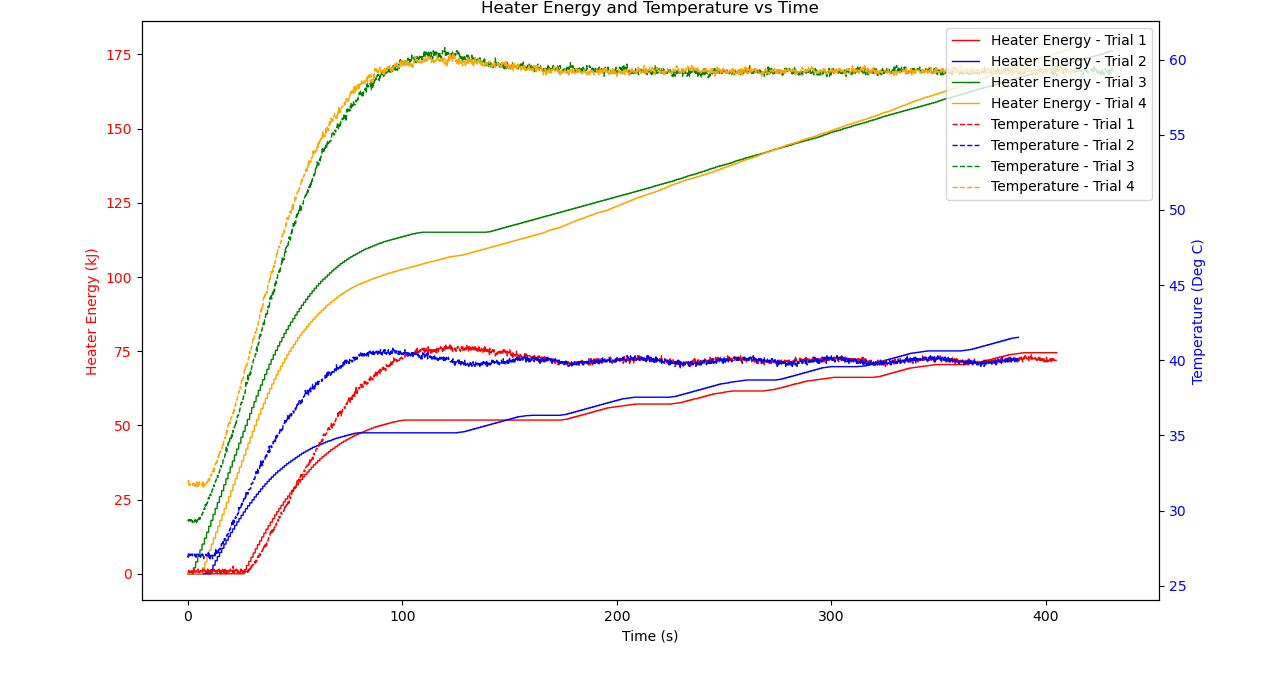
\includegraphics[width=1\linewidth]{figure/heater.png}
\caption{Plot of heater energy and temperature throughout four trials. Note that the slope of the heater energy becomes constant when the temperature becomes constant, symbolizing a steady state. This is the region we will use to calculate heater power. The non-constant slope region will be used to calculate specific heat under constant volume, $c_v$.}
\label{fig:heater}
\end{figure}
\begin{equation}
    \dot{Q}_{\rm wall}=2k_{\rm acrylic}\pi l\frac{\Delta T}{\ln\left(\frac{r_2}{r_1}\right)}
    \label{eq:heatlosswall}
\end{equation}
\begin{align*}
    \text{where } 
    &k_{\rm acrylic} = 0.185\pm0.015\left[\frac{W}{mK}\right],\;l=0.286\pm0.003[m],\;\Delta T=\frac{1}{n}\sum_i^n T_{\rm gas}-T_{\rm wall},\\
    \text{and }&r_1=0.1937\pm0.0014[m]\text{ and }r_2=0.2032\pm0.0011[m]
\end{align*}
and that the difference between the power required to maintain the temperature in the tank and the heat loss of the walls will be equal to the heat loss of the plates, according to the First Law and conservation of energy:
\begin{equation}
    \dot{W}+\dot{Q}_{\rm wall}+\dot{Q}_{\rm plates}=\Delta E = 0\implies\boxed{\dot{Q}_{\rm plates}=-\dot{W}-\dot{Q}_{\rm wall}}
    \label{eq:heatloss}
\end{equation}
Using equation (\ref{eq:heatlosswall}) and this relation, calculated results are recorded in Table \ref{table:heatloss} (where we define our system to be the gas inside the tank).
\begin{table}[h]
  \centering
  \begin{tabular}{|c|c|c|c|}
    \hline
    Trial & $\dot{W}[W]$ & $\dot{Q}_{\rm wall}[W]$ & $\dot{Q}_{\rm plates}[W]$ \\
    \hline
    1 & $94.152\pm0.005$&$ -83.23\pm60.09$&$ -10.92\pm7.86$\\
    2 & $125.484\pm0.005$&$ -77.92\pm55.94$&$ -47.56\pm33.55$\\
    3 & $198.145\pm0.005$&$ -172.93\pm123.40$&$ -25.12\pm19.03$\\
    4 & $224.121\pm0.005$&$ -158.85\pm113.28$&$ -65.27\pm45.92$\\
    \hline
  \end{tabular}
  \caption{Calculated heat transfer values (from both the acrylic walls and top and bottom plates) each trial.}
  \label{table:heatloss}
\end{table}
In the computations, the conductive heat transfer coefficient for acrylic is estimated as the mean value between its maximum and minimum values. Nevertheless, this simplification is not suitable for real-world processes because of the irregular shape of the acrylic material and contributes to unaccounted sources of error. In addition, since there is no trivial way of determining the heat transfer of the tank during the heating process, we inevitably have to assume zero heat transfer for calculating the specific heat for constant volume, $c_v$. We can do so by rearranging the First Law into:
\begin{equation}
    W+\cancel{Q}=mc_v\Delta T\implies c_v=\frac{W}{m\Delta T}
    \label{eq:firstlawrearranged}
\end{equation}
% 0.06645, 0.021, 0.0698, 0.0206 ( for c_p)
$W$ and $\Delta T$ are both interpolated from the region of the heater energy curves where the slope is non-constant (Fig. \ref{fig:heater}). Applying equation (\ref{eq:firstlawrearranged}), the calculated $c_v$ values are $$98.6\pm6.6,\;64.4\pm1.4,\;106\pm7,\;67.2\pm1.4\left[\frac{kJ}{kgK}\right]$$ for trials 1 through 4 respectively. These values are all around 3 orders of magnitude off from the real $c_v$, and a primary reason is the fact that heat transfer is ignored, even though we just proved their significance at steady state. We can clearly see that this assumption is hugely invalid and is a big source of error with no way of quantifying. However, on the other side, the trend of increase with the increase of temperature does align with what is expected.

\subsection*{Part III:  Determining the work done by the Propeller in the Left Tank}

To determine the internal energy for an adiabatic system, we calculate the work done by the propeller by looking at the fan blade performance using pump and fan similarity equations.

\begin{equation}
    \frac{{Q}_{\rm 2}}{{Q}_{\rm 1}}=\frac{{n}_{\rm 2}}{{n}_{\rm 1}}\left(\frac{{D}_{\rm 2}}{{D}_{\rm 1}}\right)^3
    \label{eq:pump_and_fan_similarity_1}
\end{equation}

\begin{equation}
    \frac{{P}_{\rm 2}}{{P}_{\rm 1}}=\frac{{\rho}_{\rm 2}}{{\rho}_{\rm 1}}\left(\frac{{n}_{\rm 2}}{{n}_{\rm 1}}\right)^3\left(\frac{{D}_{\rm 2}}{{D}_{\rm 1}}\right)^5
    \label{eq:pump_and_fan_similarity_2}
\end{equation}

\begin{align*}
    \text{where }
    &Q_{\rm 1} = 25[cfm],\;n_{\rm 1} = 4200[rpm],\;n_{\rm 2} = 2000[rpm],\;D_{\rm 1} = 2.5'',\;D_{\rm 2} = 2.5'',\;\\
    &P_{\rm 1} = 0.001[hp] = 0.746[W],\;{\rho}_{1}=1.225[\frac{kg}{m^3}],\;{\rho}_{2}=\frac{P}{RT}
\end{align*}

Using equation (\ref{eq:pump_and_fan_similarity_1}) and the given manufacturer’s test conditions values \autocite{che}, we can calculate the work done by the propeller:
\begin{equation}
    W=t \times {P}_{\rm 2} =t \times {P}_{\rm 1} \times \frac{{\rho}_{\rm 2}}{{\rho}_{\rm 1}}\left(\frac{{n}_{\rm 2}}{{n}_{\rm 1}}\right)^3\left(\frac{{D}_{\rm 2}}{{D}_{\rm 1}}\right)^5
    \label{eq:work done by the propeller}
\end{equation}

Referring back to equation (\ref{eq:firstlawrearranged}), rearranging it, and using the values calculated in the previous parts, we can calculate the rate of rise in temperature:
\begin{equation}
    W=m c_v\Delta T\implies P=m c_v\frac{\Delta T}{t}\implies\boxed{\frac{\Delta T}{t}=\frac{{P}_{\rm 2}}{m c_v}}
    \label{eq:rate_of_rise_in_temp}
\end{equation}

\begin{table}[h]
  \centering
  \begin{tabular}{|c|c|c|c|}
    \hline
    Trial & $W[J]$ & $\frac{dT}{dt}[\frac{K}{s}]$\\
    \hline
    $1 $& $81.708\pm0.136$ & $(81.192\pm1.032) \times 10^{-6}$\\
    $2 $& $136.669\pm0.103$ & $(118.382\pm1.895) \times 10^{-6}$\\
    $3 $& $81.752\pm0.094$ & $(61.051\pm0.820) \times 10^{-6}$\\
    $4 $& $137.059\pm0.115$ & $(118.252\pm1.942) \times 10^{-6}$\\
    \hline
  \end{tabular}
  \caption{Calculated work done by the propeller and rate of rise in temperature for each trial.}
  \label{table:temp}
\end{table}

The work performed by the propeller on the system is negligible compared to the heat added. Given that the heat added is approximately 1000 times greater than the work done by the propeller, its contribution is deemed insignificant in both the process and subsequent calculations. This is proven by the minute rates of change of temperature seen in Table \ref{table:temp}. Most of the inaccuracies in these numbers are carried over by our previously calculated $c_v$ values. Moreover, we are unsure of the accuracy of the provided parameters of the setup, and while that may be a source of error, it should not alter our conclusions.

\section*{Conclusion}
In conclusion, the laboratory experiment effectively demonstrates the applicability of the first law of thermodynamics within the system. We have proven some assumptions valid, and others, not so much. 
Using the ideal gas law, the calculated values of the mass in the left tank are $25.201\pm0.150$, $46.310\pm0.275$, $29.304\pm0.176$, $41.762\pm0.248[g]$ respectively. Through calculations of heat loss, and heat conduction through cylindrical walls, the constant volume-specific heat capacity of air are $98.6\pm6.6$, $64.4\pm1.4$, $106\pm7$, $67.2\pm1.4[\frac{kJ}{kgK}]$ respectively. While we have shown that there is significant heat transfer through the boundaries of the gas cylinder, we are forced to falsely assume the lack thereof due to our inability to determine it during the heating-up process. Hence, these values deviate significantly from the expected results. Finally, using the fan similarity equations, the calculated values of the work done by a propeller are $81.708\pm0.136$, $136.669\pm0.103$, $81.752\pm0.094$, $137.059\pm0.115[J]$ respectively. By looking at the temperature change rates, which are in the magnitude of $10^{-6}\;K$, we are able to get a more vivid image of what these numbers represent.
Hence, the work performed by the propeller is negligible in comparison to the heat added to the system. Thus, by combining theoretical principles with practical experimentation, this lab successfully shows the thermodynamic concepts and their application in real-world systems, and the contrast between calculated and expected values demonstrates the validity and invalidity of some assumptions we are forced to make.

\newpage
\printbibliography
\end{document}